\documentclass[preview]{standalone}
\usepackage{amsmath}
\usepackage{amssymb}
\usepackage{stellar}
\usepackage{definitions}
\usepackage{bettelini}
\usepackage{tikz}
\usepackage{pgfplots}
\pgfplotsset{compat=1.18}
\begin{document}
\id{diffeq-gronwall-growth}
\genpage
\section{Gronwall estimates}

\begin{snippettheorem}{diffeq-gronwall-control}{Differential Gronwall estimate}
    Let \(u\in C^1(I,\realnumbers^m)\) on an interval \(I\), \(t_0\in I\),
    and suppose \(\|u'(t)\|\leq P+Q\|u(t)\|\), where \(P\geq0\), \(Q>0\).
    Then
    \[
        \|u(t)\|\leq
        \left(\frac PQ+\|u(t_0)\|\right)e^{Q|t-t_0|}-\frac PQ.
    \]
    Omitting the last negative term gives a weaker bound.
    For \(Q=0\), the bound is \(\|u(t)\|\leq\|u(t_0)\|+P|t-t_0|\).
\end{snippettheorem}

\begin{snippet}{diffeq-gronwall-regularization}
    The comparison equation \(v'=P+Qv\), \(v(t_0)=\|u(t_0)\|\), has solution
    \(v=(P/Q+\|u(t_0)\|)e^{Q(t-t_0)}-P/Q\) for \(t\geq t_0\).
    Direct differentiation of a norm at zero is problematic.
    The original proof avoids it by smoothing the absolute value.
\begin{center}
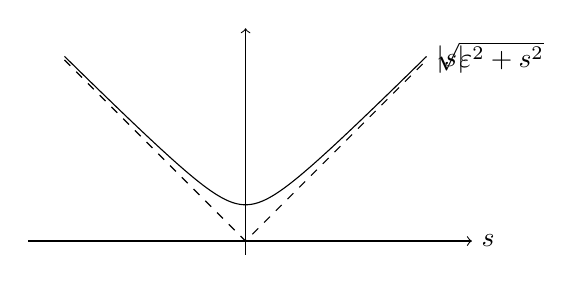
\begin{tikzpicture}[x=1.15cm,y=1.15cm]
	\draw[->] (-2.4,0) -- (2.5,0) node[right] {\(s\)};
	\draw[->] (0,-0.15) -- (0,2.35);
	\draw[dashed] (-2,2) -- (0,0) -- (2,2) node[right] {\(|s|\)};
	\draw[domain=-2:2,samples=100,smooth,variable=\s]
		plot ({\s},{sqrt(0.16+\s*\s)})
		node[right] {\(\sqrt{\varepsilon^2+s^2}\)};
\end{tikzpicture}
\end{center}
\end{snippet}

\begin{snippetproof}{diffeq-gronwall-control-proof}{diffeq-gronwall-control}{Differential Gronwall estimate}
    Set \(z_\varepsilon(t)=\sqrt{\varepsilon^2+\|u(t)\|^2}\), \(\varepsilon>0\).
    With the Euclidean inner product,
    \[
        z_\varepsilon'=\frac{\langle u,u'\rangle}{z_\varepsilon},\qquad
        |z_\varepsilon'|\leq\frac{\|u\|}{z_\varepsilon}\|u'\|
        \leq P+Q\|u\|\leq P+Qz_\varepsilon.
    \]
    Hence
    \[
        \left|\frac d{dt}\log(P+Qz_\varepsilon)\right|
        =\frac{Q|z_\varepsilon'|}{P+Qz_\varepsilon}\leq Q.
    \]
    Integrating between \(t_0\) and \(t\) gives
    \[
        \left|\log\frac{P+Qz_\varepsilon(t)}{P+Qz_\varepsilon(t_0)}\right|
        \leq Q|t-t_0|.
    \]
    Exponentiation yields
    \(z_\varepsilon(t)\leq(P/Q+z_\varepsilon(t_0))e^{Q|t-t_0|}-P/Q\).
    Let \(\varepsilon\to0\). The scalar proof is the same with
    \(\langle u,u'\rangle=uu'\). For \(Q=0\), integrate \(\|u'\|\leq P\).
\end{snippetproof}

\begin{snippetlemma}{diffeq-integral-gronwall}{Integral Gronwall inequality}
    Let \(v\geq0\) be continuous on \([a,b]\). If \(A,L\geq0\) and
    \(v(t)\leq A+L\int_a^t v(s)\,ds\), then \(v(t)\leq Ae^{L(t-a)}\).
\end{snippetlemma}

\begin{snippetproof}{diffeq-integral-gronwall-proof}{diffeq-integral-gronwall}{Integral Gronwall inequality}
    Put \(w(t)=A+L\int_a^t v(s)\,ds\). Then \(v\leq w\), \(w'\leq Lw\).
    Consequently \((e^{-L(t-a)}w)'\leq0\), giving \(v\leq w\leq Ae^{L(t-a)}\).
\end{snippetproof}

\begin{snippetproposition}{diffeq-scalar-comparison}{Scalar comparison}
    Let \(f_1,f_2\in C(I\times\realnumbers)\) be locally Lipschitz in the state,
    uniformly locally in time, and suppose \(f_1(t,y)\leq f_2(t,y)\).
    If \(y_i'=f_i(t,y_i)\) and \(y_1(t_0)=y_2(t_0)\), then
    \(y_1(t)\leq y_2(t)\) at all common times \(t\geq t_0\).
\end{snippetproposition}

\begin{snippetproof}{diffeq-scalar-comparison-proof}{diffeq-scalar-comparison}{Scalar comparison}
    On a compact common time interval take a uniform state Lipschitz constant
    \(L\) for \(f_2\) on a rectangle containing both graphs.
    For \(d=y_1-y_2\), wherever \(d>0\),
    \(d'\leq f_2(t,y_1)-f_2(t,y_2)\leq Ld\).
    At \(d=0\), \(d'\leq0\). The positive part \(d_+=\max(d,0)\)
    is absolutely continuous and satisfies \(d_+'\leq Ld_+\) almost everywhere.
    Integrating and applying Gronwall with zero initial value gives \(d_+=0\).
\end{snippetproof}

\section{Global existence under linear growth}

\begin{snippettheorem}{diffeq-linear-growth-global}{Global existence under linear growth}
    Let \(I\) be open and \(f\in C(I\times\realnumbers^m,\realnumbers^m)\).
    Suppose continuous \(a,b\colon I\fromto[0,+\infty)\) satisfy
    \[
        \|f(t,y)\|\leq a(t)+b(t)\|y\|.
    \]
    Every local solution extends to all of \(I\).
    If \(f\) is locally Lipschitz in the state, uniformly locally in time,
    every initial value problem has a unique global solution.
\end{snippettheorem}

\begin{snippetproof}{diffeq-linear-growth-global-proof}{diffeq-linear-growth-global}{Global existence under linear growth}
    Peano gives a local solution, and take any maximal extension.
    On a compact \(J\subset I\) containing the initial time put
    \(P=\max_J a\), \(Q=\max_J b\). Along the solution,
    \(\|y'\|\leq P+Q\|y\|\).
    Gronwall bounds \(\|y(t)\|\) on its intersection with \(J\);
    use the \(Q=0\) case when needed.
    A finite maximal endpoint interior to \(I\) would force the norm to infinity
    by the full-strip blow-up alternative, contradicting this bound.
    Thus every maximal extension has domain \(I\).
    Local Lipschitz continuity is needed only for uniqueness.
\end{snippetproof}

\begin{snippetnote}{diffeq-linear-growth-not-necessary}{A sufficient condition, not a necessary one}
    An at-most-linear bound prevents finite-time blow-up without requiring
    global Lipschitz continuity. It is sufficient, not necessary for global
    existence. Conversely smoothness alone does not prevent blow-up.
    For example \(y'=y^2\), \(y(0)=1\), has the maximal solution
    \(y(t)=1/(1-t)\) on \((-\infty,1)\).
\end{snippetnote}

\begin{snippetexample}{diffeq-cubic-time-blowup}{Smooth coefficients and finite-time blow-up}
    For \(y'=xy^3\), the zero solution is global. For \(y(x_0)=y_0\neq0\),
    \[
        \int_{y_0}^{y(x)}t^{-3}\,dt=\frac{x^2-x_0^2}{2},\qquad
        -\frac1{y(x)^2}+\frac1{y_0^2}=x^2-x_0^2.
    \]
    Thus
    \[
        y(x)=\frac{\operatorname{sign}(y_0)}
                   {\sqrt{y_0^{-2}+x_0^2-x^2}},
        \qquad |x|<\sqrt{y_0^{-2}+x_0^2}.
    \]
    Although \(f(x,y)=xy^3\) is smooth on the entire plane,
    its superlinear growth permits two finite blow-up endpoints.
\end{snippetexample}

\begin{snippetexample}{diffeq-bounded-sine-global}{Bounded but not globally Lipschitz}
    The equation \(y'=\sin(y^2)\) has \(|f|\leq1\), so all solutions are global.
    Its state derivative \(2y\cos(y^2)\) is unbounded, so \(f\) is not globally
    Lipschitz. It is locally smooth, which still gives uniqueness.
    More generally any bounded continuous vector field on a full strip
    has global extensions; local Lipschitz continuity adds uniqueness.
\end{snippetexample}

\begin{snippetexample}{diffeq-square-root-growth}{Global existence without uniqueness}
    For \(y'=\sqrt{|y|}\), the right-hand side is uniformly continuous but
    not locally Lipschitz at zero. Nevertheless
    \(\sqrt{|y|}\leq1+|y|\), so all local solutions have global extensions.
    At zero there are waiting-time solutions, for example
    \(y=0\) for \(t\leq c\), \(y=(t-c)^2/4\) for \(t>c\).
\end{snippetexample}

\end{document}
